\documentclass[10pt,border=2pt]{standalone}
\usepackage[T1]{fontenc}
\usepackage{helvet}
\renewcommand{\familydefault}{\sfdefault}
\usepackage{xcolor}
\usepackage{url}
\usepackage{array}
\usepackage{tikz}
\usetikzlibrary{positioning,arrows.meta,calc}
\newcommand{\searchDate}{2026-10-05}
\newcommand{\ieeeDate}{2026-10-05}
\newcommand{\openalexDate}{2026-10-06}
\newcommand{\chaseDate}{2026-10-06}
\newcommand{\nScopusRawA}{719}
\newcommand{\nScopusA}{528}
\newcommand{\nWoSRawA}{426}
\newcommand{\nWoSA}{399}
\newcommand{\nIEEERawA}{832}
\newcommand{\nIEEEA}{399}
\newcommand{\nOpenAlexRawA}{475}
\newcommand{\nOpenAlexA}{219}
\newcommand{\nIdentifiedA}{1545}
\newcommand{\nUniqueA}{906}
\newcommand{\nTAScreenedA}{906}
\newcommand{\nDuplicatesA}{639}
\newcommand{\nTAExcludedA}{852}
\newcommand{\nSoughtA}{54}
\newcommand{\nNotRetrievedA}{0}
\newcommand{\nFullTextA}{54}
\newcommand{\nFTxIoneA}{0}
\newcommand{\nFTxItwoA}{13}
\newcommand{\nFTxIthreeA}{3}
\newcommand{\nFTxIfourA}{0}
\newcommand{\nFTxEoneA}{9}
\newcommand{\nFTxEtwoA}{2}
\newcommand{\nFTxEthreeA}{8}
\newcommand{\nFTxEfourA}{1}
\newcommand{\nFTxEfiveA}{0}
\newcommand{\nFTxADA}{1}
\newcommand{\nFTExcludedA}{37}
\newcommand{\nIncludedDbA}{17}
\newcommand{\nCitChaseA}{588}
\newcommand{\nKnownA}{3}
\newcommand{\nOtherRemovedA}{6}
\newcommand{\nOtherScreenedA}{585}
\newcommand{\nOtherSoughtA}{4}
\newcommand{\nOtherTAExcludedA}{581}
\newcommand{\nOtherNotRetrievedA}{0}
\newcommand{\nOtherAssessedA}{4}
\newcommand{\nOxIoneA}{0}
\newcommand{\nOxItwoA}{0}
\newcommand{\nOxIthreeA}{2}
\newcommand{\nOxIfourA}{1}
\newcommand{\nOxEoneA}{1}
\newcommand{\nOxEtwoA}{0}
\newcommand{\nOxEthreeA}{0}
\newcommand{\nOxEfourA}{0}
\newcommand{\nOxEfiveA}{0}
\newcommand{\nOxADA}{0}
\newcommand{\nOtherExcludedA}{4}
\newcommand{\nOtherMethodsA}{0}
\newcommand{\nIncludedA}{17}
\newcommand{\nIncludedAone}{10}
\newcommand{\nIncludedAtwo}{7}
\newcommand{\packageURL}{\href{https://github.com/MOHAMMED-ABDALSALAM-PG/SWR-HPC-systematic-review}{\mbox{\nolinkurl{https://github.com/}}\allowbreak\mbox{\nolinkurl{MOHAMMED-ABDALSALAM-PG/}}\hspace{0pt plus 1fil}\penalty0\hspace{0pt plus -1fil}\mbox{\nolinkurl{SWR-HPC-systematic-review}}}}

\providecommand{\packageURL}{\href{https://github.com/MOHAMMED-ABDALSALAM-PG/SWR-HPC-systematic-review}{\mbox{\nolinkurl{https://github.com/}}\allowbreak\mbox{\nolinkurl{MOHAMMED-ABDALSALAM-PG/}}\hspace{0pt plus 1fil}\penalty0\hspace{0pt plus -1fil}\mbox{\nolinkurl{SWR-HPC-systematic-review}}}}
\providecommand{\chaseDate}{\textbf{\textcolor{red}{[pending]}}}
\providecommand{\ieeeDate}{\textbf{\textcolor{red}{[pending]}}}
\providecommand{\nCitChaseA}{\textbf{\textcolor{red}{[pending]}}}
\providecommand{\nFTxEfiveA}{\textbf{\textcolor{red}{[pending]}}}
\providecommand{\nFTxADA}{\textbf{\textcolor{red}{[pending]}}}
\providecommand{\nFTxEfourA}{\textbf{\textcolor{red}{[pending]}}}
\providecommand{\nFTxEoneA}{\textbf{\textcolor{red}{[pending]}}}
\providecommand{\nFTxEthreeA}{\textbf{\textcolor{red}{[pending]}}}
\providecommand{\nFTxEtwoA}{\textbf{\textcolor{red}{[pending]}}}
\providecommand{\nFTxIfourA}{\textbf{\textcolor{red}{[pending]}}}
\providecommand{\nFTxIoneA}{\textbf{\textcolor{red}{[pending]}}}
\providecommand{\nFTxIthreeA}{\textbf{\textcolor{red}{[pending]}}}
\providecommand{\nFTxItwoA}{\textbf{\textcolor{red}{[pending]}}}
\providecommand{\nIEEERawA}{\textbf{\textcolor{red}{[pending]}}}
\providecommand{\nIEEERawB}{\textbf{\textcolor{red}{[pending]}}}
\providecommand{\nIncludedB}{\textbf{\textcolor{red}{[pending]}}}
\providecommand{\nNotRetrievedA}{\textbf{\textcolor{red}{[pending]}}}
\providecommand{\nOtherAssessedA}{\textbf{\textcolor{red}{[pending]}}}
\providecommand{\nOtherExcludedA}{\textbf{\textcolor{red}{[pending]}}}
\providecommand{\nOtherNotRetrievedA}{\textbf{\textcolor{red}{[pending]}}}
\providecommand{\nOtherRemovedA}{\textbf{\textcolor{red}{[pending]}}}
\providecommand{\nOtherScreenedA}{\textbf{\textcolor{red}{[pending]}}}
\providecommand{\nOtherSoughtA}{\textbf{\textcolor{red}{[pending]}}}
\providecommand{\nOtherTAExcludedA}{\textbf{\textcolor{red}{[pending]}}}
\providecommand{\nOxEfiveA}{\textbf{\textcolor{red}{[pending]}}}
\providecommand{\nOxADA}{\textbf{\textcolor{red}{[pending]}}}
\providecommand{\nOxEfourA}{\textbf{\textcolor{red}{[pending]}}}
\providecommand{\nOxEoneA}{\textbf{\textcolor{red}{[pending]}}}
\providecommand{\nOxEthreeA}{\textbf{\textcolor{red}{[pending]}}}
\providecommand{\nOxEtwoA}{\textbf{\textcolor{red}{[pending]}}}
\providecommand{\nOxIfourA}{\textbf{\textcolor{red}{[pending]}}}
\providecommand{\nOxIoneA}{\textbf{\textcolor{red}{[pending]}}}
\providecommand{\nOxIthreeA}{\textbf{\textcolor{red}{[pending]}}}
\providecommand{\nOxItwoA}{\textbf{\textcolor{red}{[pending]}}}
\providecommand{\nScalarizedB}{\textbf{\textcolor{red}{[pending]}}}
\providecommand{\nScreenedB}{\textbf{\textcolor{red}{[pending]}}}
\providecommand{\nFullTextB}{\textbf{\textcolor{red}{[pending]}}}
\providecommand{\nSoughtA}{\textbf{\textcolor{red}{[pending]}}}
\providecommand{\nKnownA}{\textbf{\textcolor{red}{[pending]}}}
\providecommand{\openalexDate}{\textbf{\textcolor{red}{[pending]}}}

\definecolor{prismaDark}{HTML}{1F4E79}
\definecolor{prismaMid}{HTML}{2E75B6}
\definecolor{prismaLight}{HTML}{DEEBF7}
\definecolor{prismaPale}{HTML}{F3F8FD}
\definecolor{hdrFill}{HTML}{FFC000}
\definecolor{hdrLine}{HTML}{7F6000}
\definecolor{stageFill}{HTML}{9DC3E6}
% exclusion reasons: code and short label | count
\newcommand{\reasons}[9]{%
  \begin{tabular*}{\linewidth}{@{}l@{\hspace{3pt}}l@{\extracolsep{\fill}}r@{}}
  I1 & Not primary/English & #1\\
  I2 & No weather/ocean field & #2\\
  I3 & No parallel scheme & #3\\
  I4 & No performance result & #4\\
  E1 & Parallelism only named & #5\\
  E2 & HPC not for the routing & #6\\
  E3 & Not route planning & #7\\
  E4 & Review, thesis or similar & #8\\
  E5 & Additional report & #9\\
  -- & Author decision & \reasonsAD
  \end{tabular*}}
\hyphenpenalty=10000 \exhyphenpenalty=10000
\begin{document}
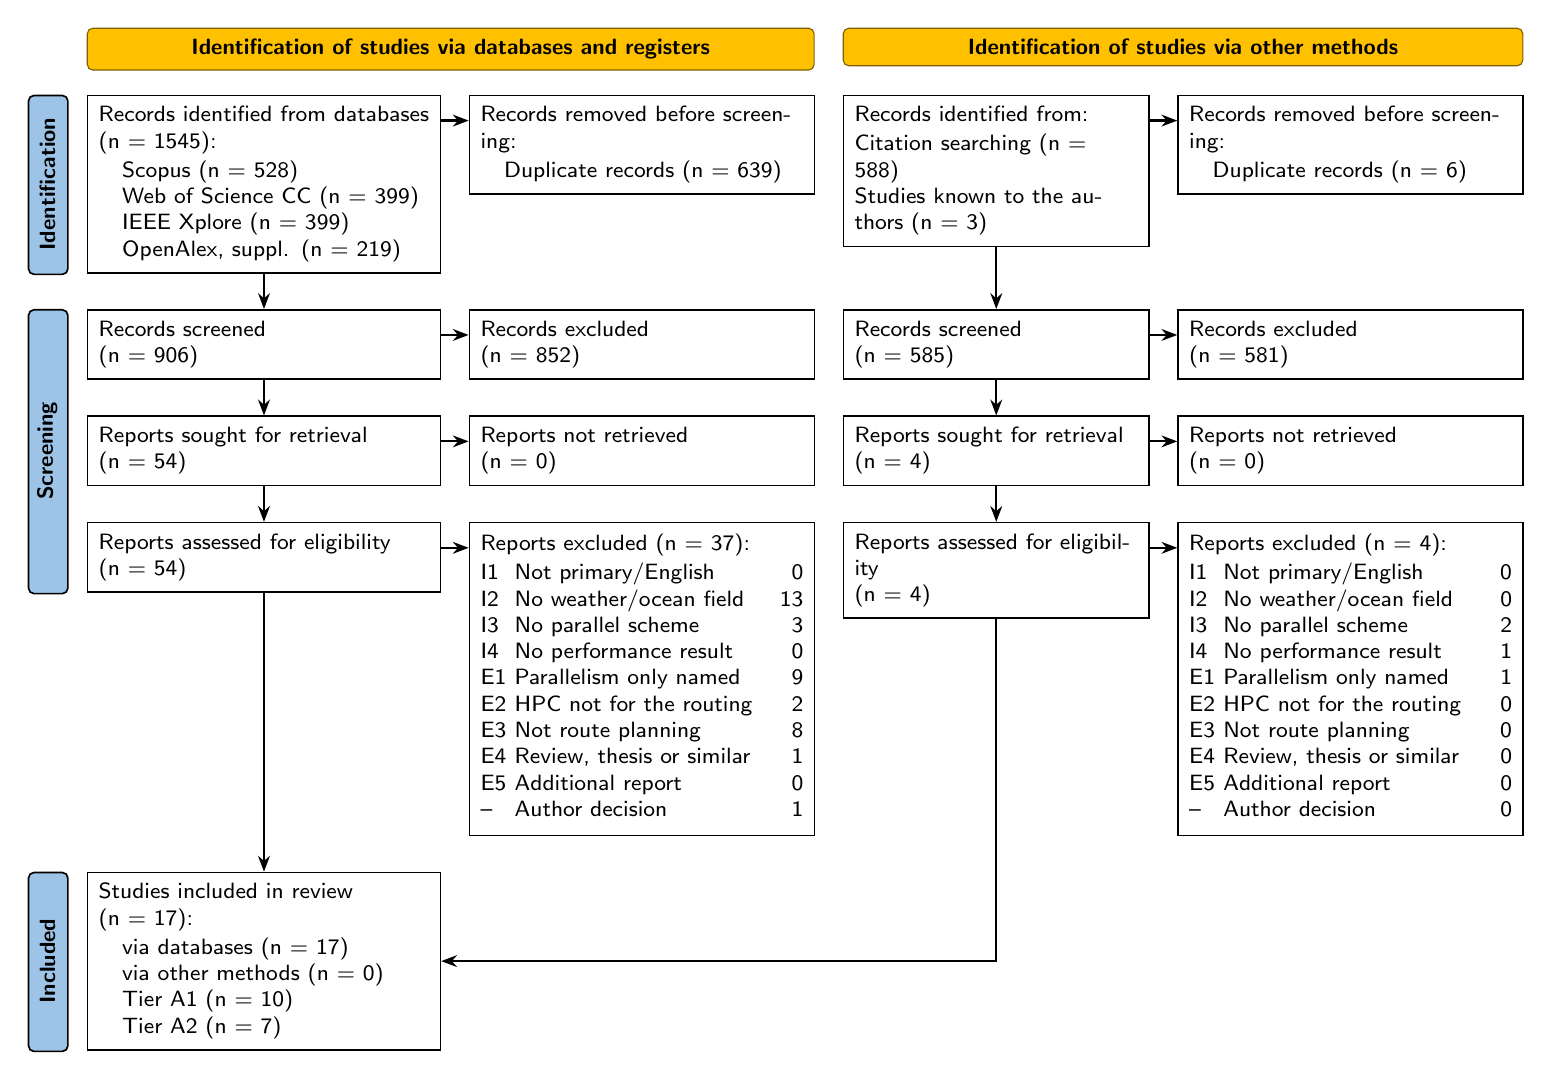
\begin{tikzpicture}[
  font=\footnotesize,
  box/.style={draw=black, fill=white, line width=0.6pt, rectangle, align=left, text width=#1, inner sep=4pt, anchor=north west},
  box/.default=3.7cm,
  hdr/.style={draw=hdrLine, line width=0.4pt, rectangle, rounded corners=2pt, fill=#1, text=black, align=center, inner sep=4pt, font=\footnotesize\bfseries, anchor=north west},
  hdr/.default=hdrFill,
  stage/.style={draw=black, fill=stageFill, rounded corners=2pt, line width=0.6pt},
  arr/.style={-{Stealth[length=2mm]}, thick, draw=black}
]
\def\xL{0.75}  \def\wL{4.2cm}
\def\xLs{5.6} \def\wLs{4.1cm}
\def\xR{10.35}  \def\wR{3.6cm}
\def\xRs{14.6} \def\wRs{4.1cm}
\def\gap{0.45}
% next row starts below the lowest of the four boxes of the previous row
\newcommand{\rowbelow}[5]{\path let \p1=(#1.south), \p2=(#2.south), \p3=(#3.south), \p4=(#4.south)
  in coordinate (#5) at (0, {min(min(\y1,\y2),min(\y3,\y4)) - \gap cm});}
\node[hdr, text width=8.95cm] (hL) at (\xL,0) {Identification of studies via databases and registers};
\node[hdr, text width=8.35cm] (hR) at (\xR,0) {Identification of studies via other methods};
\coordinate (y1) at (0,-0.85);
\node[box=\wL]  (L1)  at (\xL,0 |- y1) {Records identified from databases (n = \nIdentifiedA):\\[1pt]
  \quad Scopus (n = \nScopusA)\\ \quad Web of Science CC (n = \nWoSA)\\ \quad IEEE Xplore (n = \nIEEEA)\\ \quad OpenAlex, suppl. (n = \nOpenAlexA)};
\node[box=\wLs] (L1s) at (\xLs,0 |- y1) {Records removed before screening:\\[1pt] \quad Duplicate records (n = \nDuplicatesA)};
\node[box=\wR]  (R1)  at (\xR,0 |- y1) {Records identified from:\\[1pt] Citation searching (n = \nCitChaseA)\\ Studies known to the authors (n = \nKnownA)};
\node[box=\wRs] (R1s) at (\xRs,0 |- y1) {Records removed before screening:\\[1pt] \quad Duplicate records (n = \nOtherRemovedA)};
\rowbelow{L1}{L1s}{R1}{R1s}{y2}
\node[box=\wL]  (L2)  at (\xL,0 |- y2) {Records screened\\ (n = \nUniqueA)};
\node[box=\wLs] (L2s) at (\xLs,0 |- y2) {Records excluded\\ (n = \nTAExcludedA)};
\node[box=\wR]  (R2)  at (\xR,0 |- y2) {Records screened\\ (n = \nOtherScreenedA)};
\node[box=\wRs] (R2s) at (\xRs,0 |- y2) {Records excluded\\ (n = \nOtherTAExcludedA)};
\rowbelow{L2}{L2s}{R2}{R2s}{y3}
\node[box=\wL]  (L3)  at (\xL,0 |- y3) {Reports sought for retrieval\\ (n = \nSoughtA)};
\node[box=\wLs] (L3s) at (\xLs,0 |- y3) {Reports not retrieved\\ (n = \nNotRetrievedA)};
\node[box=\wR]  (R3)  at (\xR,0 |- y3) {Reports sought for retrieval\\ (n = \nOtherSoughtA)};
\node[box=\wRs] (R3s) at (\xRs,0 |- y3) {Reports not retrieved\\ (n = \nOtherNotRetrievedA)};
\rowbelow{L3}{L3s}{R3}{R3s}{y4}
\node[box=\wL]  (L4)  at (\xL,0 |- y4) {Reports assessed for eligibility\\ (n = \nFullTextA)};
\def\reasonsAD{\nFTxADA}
\node[box=\wLs] (L4s) at (\xLs,0 |- y4) {Reports excluded (n = \nFTExcludedA):\\[1pt]
  \reasons{\nFTxIoneA}{\nFTxItwoA}{\nFTxIthreeA}{\nFTxIfourA}{\nFTxEoneA}{\nFTxEtwoA}{\nFTxEthreeA}{\nFTxEfourA}{\nFTxEfiveA}};
\node[box=\wR]  (R4)  at (\xR,0 |- y4) {Reports assessed for eligibility\\ (n = \nOtherAssessedA)};
\def\reasonsAD{\nOxADA}
\node[box=\wRs] (R4s) at (\xRs,0 |- y4) {Reports excluded (n = \nOtherExcludedA):\\[1pt]
  \reasons{\nOxIoneA}{\nOxItwoA}{\nOxIthreeA}{\nOxIfourA}{\nOxEoneA}{\nOxEtwoA}{\nOxEthreeA}{\nOxEfourA}{\nOxEfiveA}};
\rowbelow{L4}{L4s}{R4}{R4s}{y5}
\node[box=\wL] (L5) at (\xL,0 |- y5) {Studies included in review\\ (n = \nIncludedA):\\[1pt]
  \quad via databases (n = \nIncludedDbA)\\ \quad via other methods (n = \nOtherMethodsA)\\ \quad Tier A1 (n = \nIncludedAone)\\ \quad Tier A2 (n = \nIncludedAtwo)};
% stage bars
\foreach \a/\b/\t in {L1/L1/Identification, L2/L4/Screening, L5/L5/Included}{
  \path let \p1=(\a.north), \p2=(\b.south) in
    node[stage, minimum width=0.5cm, minimum height={\y1-\y2}, anchor=north west] at (0,\y1) {}
    node[rotate=90, font=\footnotesize\bfseries, text=black] at (0.25,{(\y1+\y2)/2}) {\t};}
% arrows
\foreach \m/\s in {L1/L1s,L2/L2s,L3/L3s,L4/L4s,R1/R1s,R2/R2s,R3/R3s,R4/R4s}{
  \draw[arr] ($(\m.north east)+(0,-0.33)$) -- ($(\s.north west)+(0,-0.33)$);}
\foreach \a/\b in {L1/L2,L2/L3,L3/L4,L4/L5,R1/R2,R2/R3,R3/R4}{\draw[arr] (\a.south) -- (\a.south |- \b.north);}
\draw[arr] (R4.south) |- (L5.east);
\end{tikzpicture}
\end{document}
